\chapter{Operational Amplifiers}

\section{Basic Configuration}

\section{Non-inverting}
\begin{figure}[H]
	\centering
	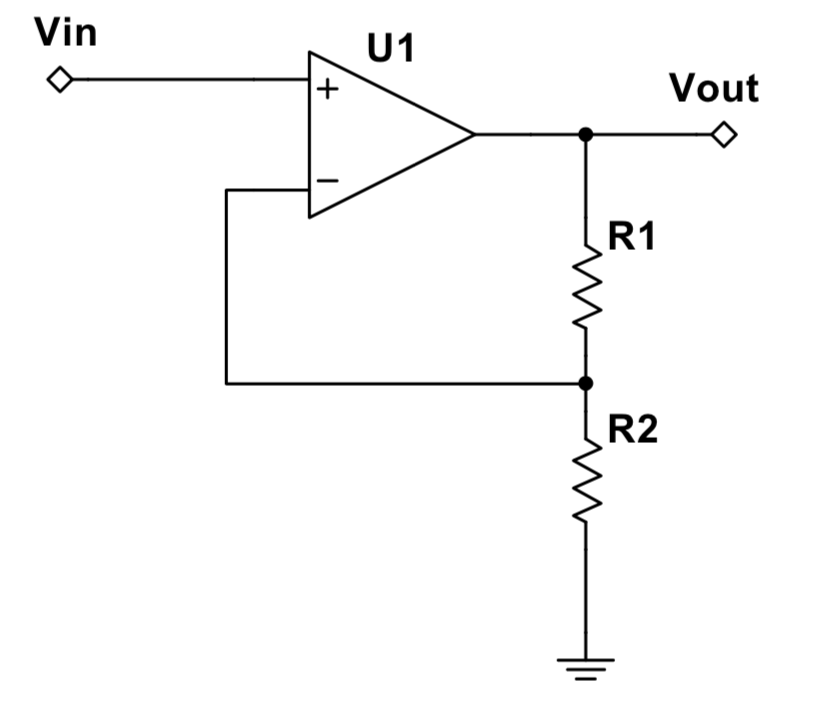
\includegraphics[width=2in]{opamps/noninverting.png}
%	\caption{Non-inverting}
	\label{fig:fig}
\end{figure}
Gain equation:
\[\frac{V_{out}}{V_{in}} = \frac{R_2 + R_1}{R_2} \]
%\begin{figure}
%	\begin{center}
%		\begin{circuitikz}
%			\draw (0,0) node[op amp] (opamp) {}
%			(opamp.-) to [R, l_=$R_1$, *-o] ($(opamp.-)-(2,0)$) node[left]{$V_{in}$}
%			(opamp.-) |- ($(opamp.-)+(0.2,1)$) to[R=$R_2$] ($(opamp.-)+(2.2,1)$) -|
%			(opamp.out) to[short,*-] ($(opamp.out)+(.5,0)$) node [right] {$V_{out}$} node [ocirc] {} 
%			(opamp.+) to[short]  ($(opamp.+)-(0,.5)$) node[ground] {}
%			;
%		\end{circuitikz}
%	\end{center}
%\end{figure}

\section{Inverting}
\begin{figure}[H]
	\centering
	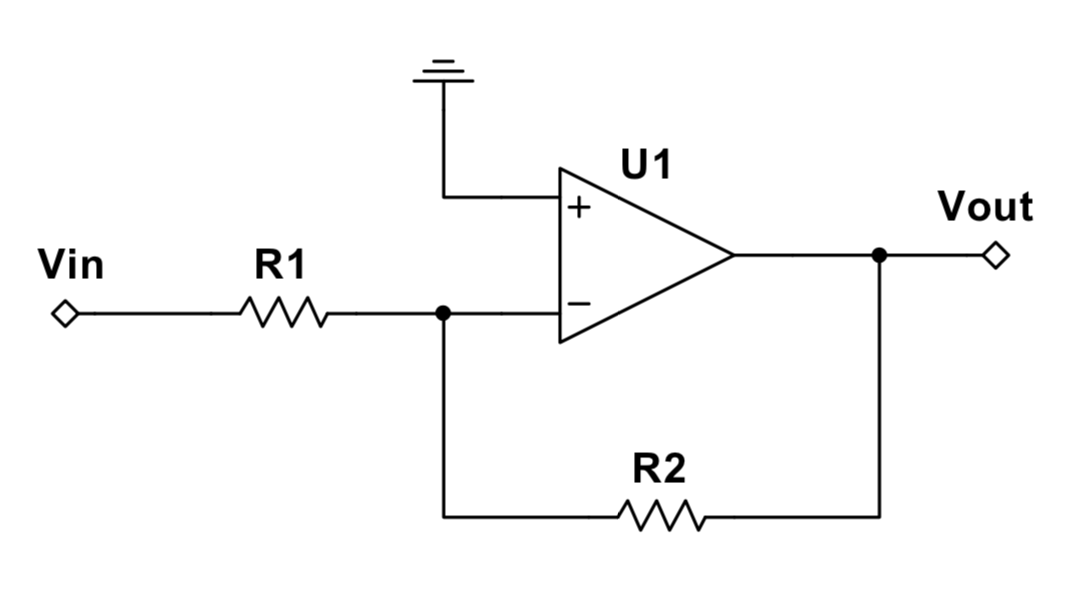
\includegraphics[width=2in]{opamps/inverting.png}
%	\caption{Inverting}
	\label{fig:fig}
\end{figure}
Gain equation:
\[\frac{V_{out}}{V_{in}} = -\frac{R_2}{R_1} \]

\section{Summer}
\begin{figure}[H]
	\centering
	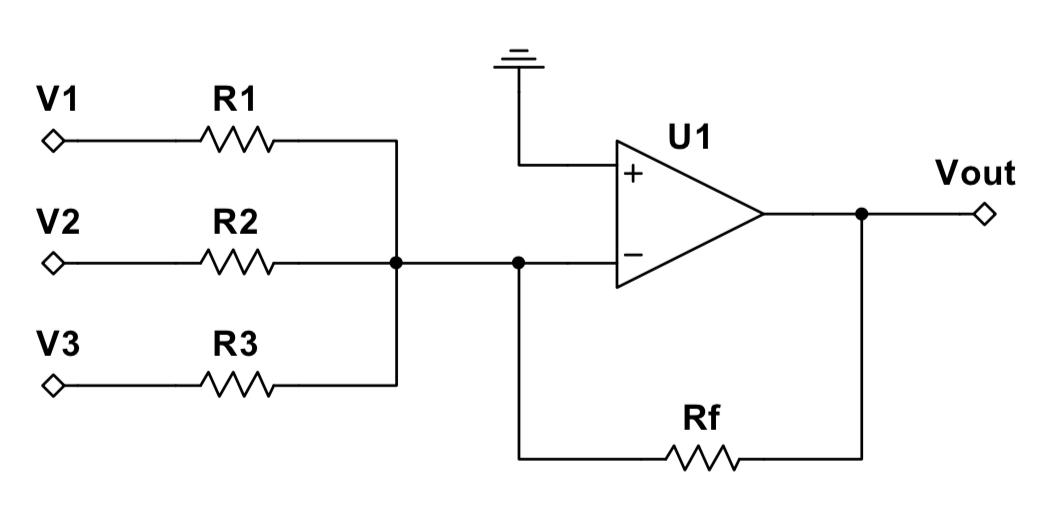
\includegraphics[width=2.5in]{opamps/summer.png}
%	\caption{Summer}
	\label{fig:fig}
\end{figure}
If $R_{in} =R_1=R_2=R_3$,
\[V_{out} = -\frac{R_f}{R_{in}}\left(V_1 + V_2 + V_3 + \cdots\right) \] 
Otherwise its a weighted summer, with equation
\[V_{out}= -\left(\frac{R_f}{R_1}V_1 + \frac{R_f}{R_2}V_2 + \cdots \frac{R_f}{R_n}V_n\right) \]


\section{Schmidt Trigger}
\begin{figure}[H]
	\centering
	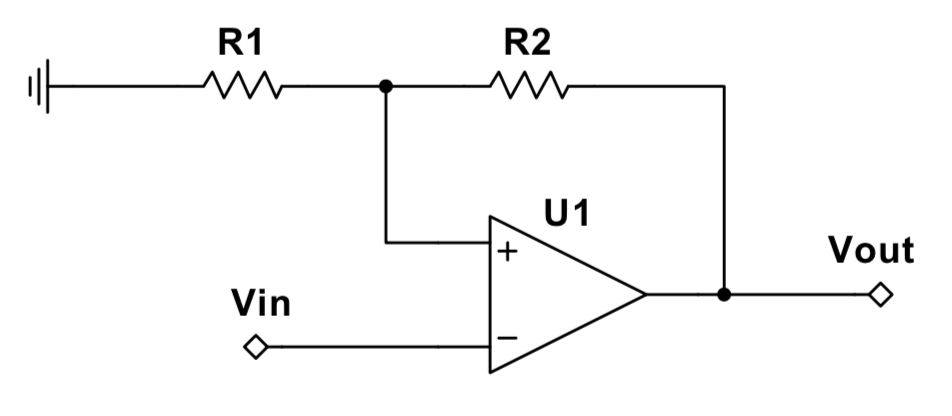
\includegraphics[width=2in]{opamps/schmidt.png}
%	\caption{Schmidt Trigger}
	\label{fig:fig}
\end{figure}
\todo{guardband}

\section{Oscillator}
\begin{figure}[H]
	\centering
	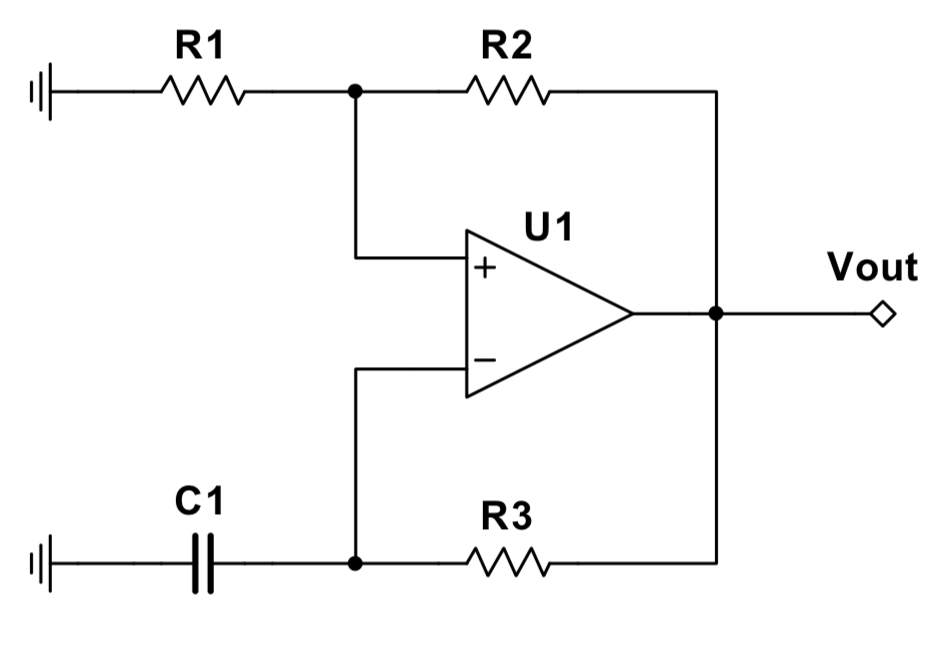
\includegraphics[width=2in]{opamps/oscillator.png}
%	\caption{Oscillator}
	\label{fig:fig}
\end{figure}
\todo{hysteresis}

\section{Integrator}
\begin{figure}[H]
	\centering
	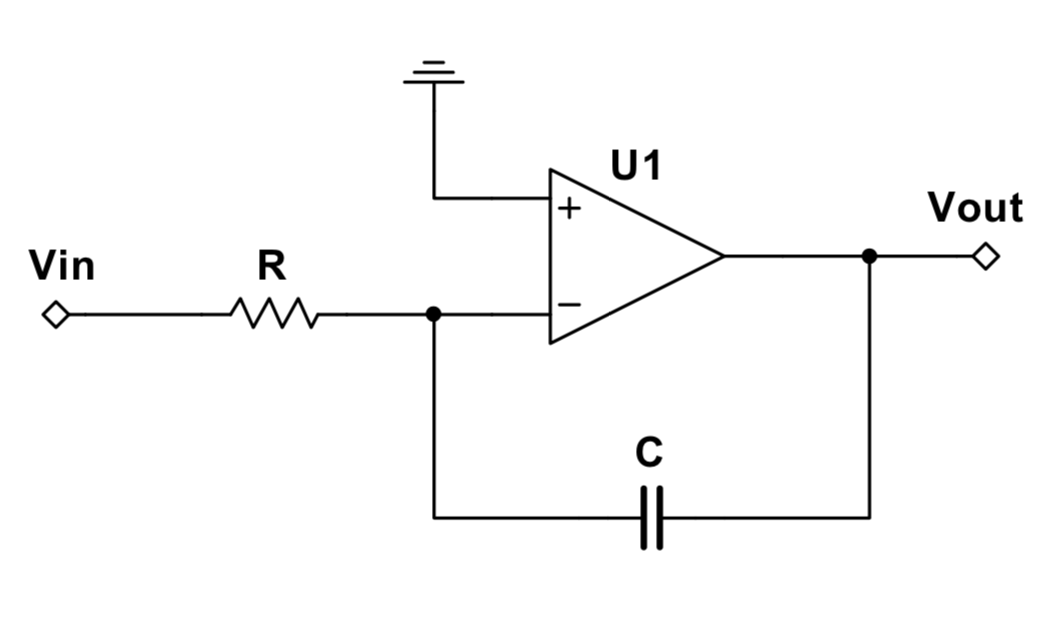
\includegraphics[width=2in]{opamps/integrator.png}
%	\caption{Integrator}
	\label{fig:fig}
\end{figure}
\[V_{out}= -\frac{1}{RC}\int_{0}^{t}V_{in}dt \]
\section{Differentiator}
\begin{figure}[H]
	\centering
	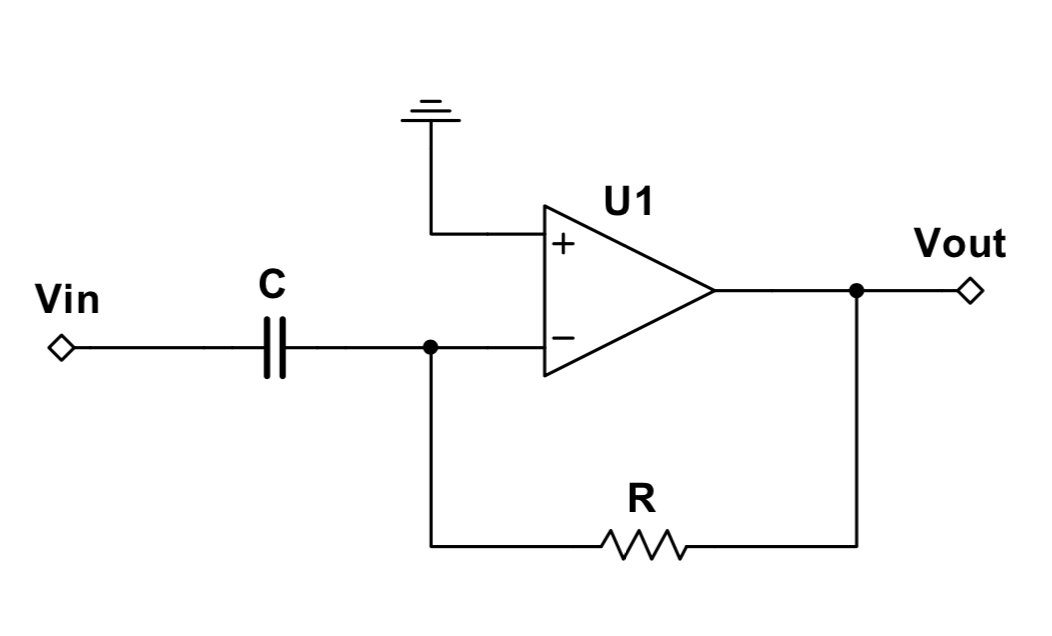
\includegraphics[width=2in]{opamps/differentiator.png}
%	\caption{Differentiator}
	\label{fig:fig}
\end{figure}
\[V_{out} = -RC\frac{dV_{in}}{dt} \]

